\documentclass[12pt, titlepage]{article}
\usepackage[english]{babel}
\usepackage[utf8]{inputenc}

\usepackage{graphicx} %graphics files inclusion
% \usepackage{subfig} %subfigures
\usepackage{amsmath} %advanced maths
\usepackage{amssymb} %additional math symbols
\usepackage{dsfont}  %contains \mathds{1}
\usepackage{algpseudocode}
\usepackage{url}

\usepackage{dirtree} %directory tree visualisation

\usepackage[draft]{todonotes}   % notes showed

\usepackage[ruled,vlined]{algorithm2e}
\newcommand\mycommfont[1]{\footnotesize\ttfamily\textcolor{blue}{#1}}
\SetCommentSty{mycommfont}

\usepackage{xcolor, colortbl}
\usepackage{pdfpages}

\newcommand{\lnorm}[1]{\left\lVert#1\right\rVert^2}
\newcommand{\norm}[1]{\left\lVert#1\right\rVert}

\algnewcommand\algorithmicforeach{\textbf{for each:}}
\algnewcommand\ForEach{\item[ \algorithmicforeach]}
\author{Radek Bartyzal}

\begin{document}
\begin{titlepage}
    \centering
    \vfill
    {\bfseries\Huge
        An Empirical Evaluation of Generic Convolutional and Recurrent Networks for Sequence Modeling \\
    }    
        \vskip1cm
        
    {\bfseries\Large 
    Czech Technical University in Prague\\ 
    Faculty of Informatics\\ 
    \vskip1cm
    Radek Bartyzal\\
    }    
    \vskip1cm
    March 5, 2019
    \vfill

    \vfill
    \vfill
\end{titlepage}

\tableofcontents

\section{Prerequisites}
The following text assumes that the reader is familiar with these terms:

\begin{itemize}
\item Neural Networks: Chapter 1 of \cite{cit:nn} 
\item Convolutional Neural Networks (CNN): \cite{cit:cnn}
\item Generic Recurrent Neural Networks (RNN): \cite{cit:lstm}
\item Long Short Term Memory Networks (LSTM): \cite{cit:lstm}
\end{itemize}

\section{Sequence Modeling}\label{sec:seq}
Suppose that we are given an input sequence $x_0, \dots , x_T$, and wish to predict some corresponding outputs $y_0, \dots , y_T$ at each time step. The key constraint, called \textbf{causal constraint}, is that to predict the output $y_t$ for some time step $t$, we are constrained to only use those inputs that have been previously observed: $x_0, \dots , x_t$. In other words the function producing $y_t$ cannot depend on future inputs $x_{t+1}, \dots, x_T.$


The goal of learning in the sequence modeling setting is to find a network $f$ that minimizes some expected loss between the actual outputs and the predictions, $L(y_0, \dots , y_T, f(x_0, \dots , x_T))$, where the sequences and outputs are drawn according to some distribution.

This formalism encompasses many settings such as \textbf{auto-regressive prediction} (where we try to predict some signal given its past) by setting the target output to be simply the input shifted by one time step. It does not, however, directly capture domains such as \textbf{machine translation}, or \textbf{sequence-to-sequence prediction} in general, since in these cases the entire input sequence (including “future” states) can be used to predict each output (though the techniques can naturally be extended to work in such settings).

\section{Temporal Convolutional Networks (TCN)}
TCN describe a family of network architectures.
The distinguishing characteristics of TCNs are: 

\begin{itemize}
\item The convolutions in the architecture are causal, meaning that there is no information “leakage” from future to past. This is achieved by \textbf{Causal convolutions}, convolutions where an output at time t is convolved only with elements from time t and earlier in the previous layer.

\item The architecture can take a sequence of any length and map it to an output sequence of the same length, just as with an RNN. This is achieved by using \textbf{1D fully-convolutional network (FCN)} architecture where each hidden layer is the same length as the input layer, and zero padding of length (kernel size $-$ 1) is added to keep subsequent layers the same length as previous ones.
\end{itemize}

Beyond this, TCNs are able to build very long effective history sizes (i.e., the ability for the networks to look very far into the past to make a prediction) using a combination of:

\begin{itemize}
\item Very deep networks augmented with \textbf{residual connections} for easier convergence.
\item \textbf{Dilated convolutions} to create exponentially larger receptive field with every added layer.
\end{itemize}

\subsection{Dilated Convolutions}
A simple causal convolution is only able to look back at a history with size linear in the depth of the network. This makes it challenging to apply it on sequence tasks requiring longer history.

Dilated convolution enables an exponentially large receptive field. More formally, for a 1-D sequence input $X \in \mathbb{R}^n$ and a filter $f:\{0, \dots , k - 1\} \rightarrow \mathbb{R}$, the dilated convolution operation $F$ on element at index $s$ of the sequence is defined as:

\begin{equation}
F(s) = \sum_{i=0}^{k-1}{f(i)X_{s - d \cdot i}}
\end{equation}

where $d$ is the dilation factor, $k$ is the filter size, and $s - d \cdot i$ represents the direction into the past. Dilation is thus equivalent to introducing a fixed step between every two adjacent filter taps. When $d=1$, a dilated convolution reduces to a regular convolution. Using larger dilation enables an output at the top level to represent a wider range of inputs, thus effectively expanding the receptive field of a ConvNet.

There are two ways to increase the receptive field of the TCN
\begin{itemize}
\item Choosing larger filter sizes $k$.
\item Increasing the dilation factor $d$.
\end{itemize}
The effective history of one such layer is
$(k - 1)d$. \\

The $d$ is increased exponentially with the depth of the network (i.e., $d = O(2^i)$ at level $i$ of the network). This ensures that there is some filter that hits each input within the effective history, while also allowing for an extremely large effective history using deep networks. An illustration is in Figure \ref{fig:diagrams}a.

\begin{figure}[h!]
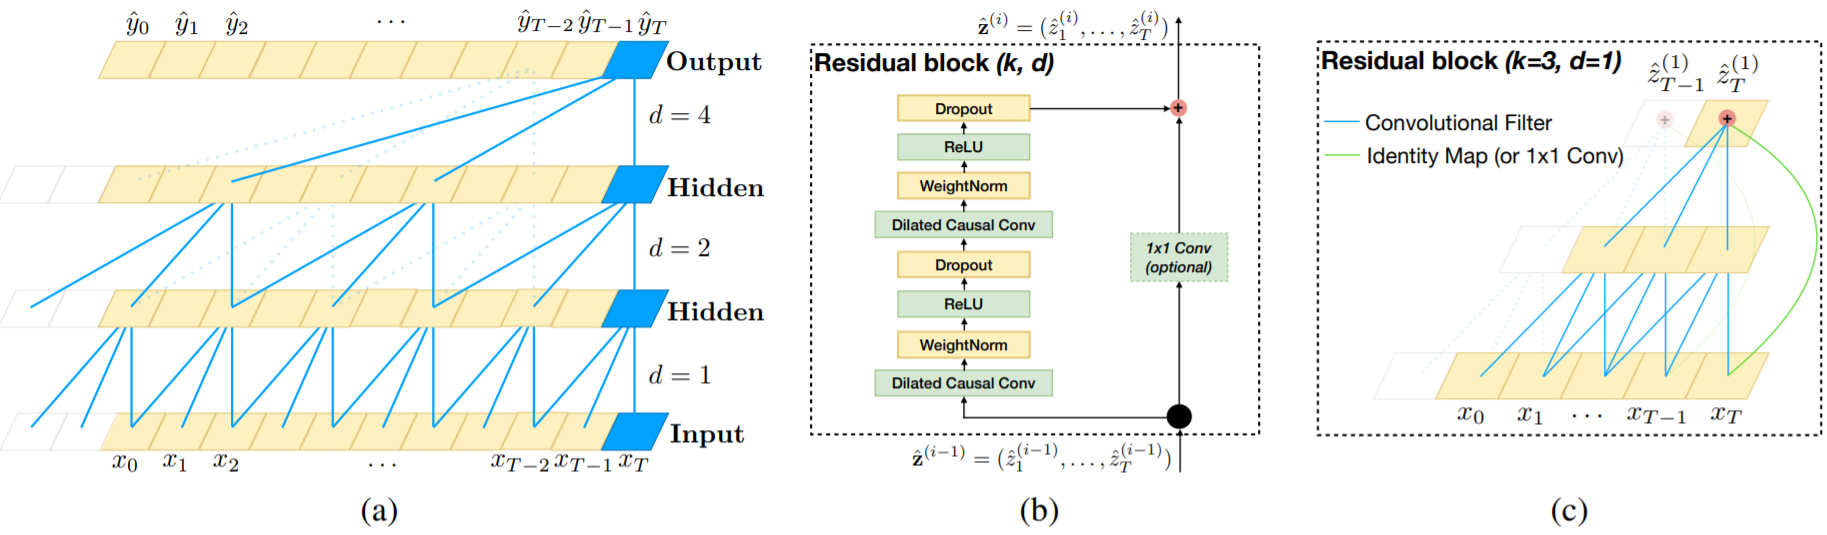
\includegraphics[width=1.0\textwidth]{../img/diagrams}
\caption{a) Dilated causal convolution with $k=3$, $d=[2^0, 2^1, 2^2]$. The receptive field is able to cover all values from the input sequence. b) TCN residual block. An 1x1 convolution is added when residual input and output have different dimensions. c) An example of residual connection in a TCN.}
\label{fig:diagrams}
\end{figure}

\subsection{Residual Connections}

A residual block contains a branch leading out to a series of transformations $F$, whose outputs are added to the input $x$ of the block:
$$o = \text{Activation}(x + F(x))$$
This effectively allows layers to learn modifications to the identity mapping rather than the entire transformation, which has repeatedly been shown to benefit very deep networks.

A generic residual module shown in Figure \ref{fig:diagrams}b is used in place of a standard convolutional layer to help convergence. It uses spatial dropout for regularization: at each training step, a whole channel is zeroed out.

In standard ResNet the input is added directly to the output of the residual function, in TCN (and ConvNets in general) the input and output could have different widths. To account for discrepant input-output widths, an additional 1x1 convolution is used to ensure that the element-wise addition receives tensors of the same shape.

\subsection{Advantages and disadvantages}

\subsubsection{Advantages}
\begin{itemize}
\item \textbf{Parallelism}: Kernels are reused = one layer can be calculated in parallel.
\item \textbf{Flexible receptive field size}: Changing receptive field by: changing: $d$, $k$, number of layers.
\item \textbf{Stable gradients}: Backpropagation path different from the temporal direction of the sequence = the error propagates only through layers not through time.
\item \textbf{Low memory requirement for training}: Kernels are reused = less memory than LSTMs that keep partial results for various gates.
\item \textbf{Variable length inputs}: TCNs can also take in inputs of arbitrary lengths by sliding the 1D convolutional kernels.
\end{itemize}

\subsubsection{Disadvantages}

\begin{itemize}
\item \textbf{Data storage during evaluation}: LSTMs need only one hidden state to predict. TCNs need whole input sequence.
\item \textbf{Potential parameter change for a transfer of domain}: If transfering to a domain with longer history dependencies, the $k$ and $d$ might need to be changed.
\end{itemize}

\section{Results}

The datasets are explained well in the paper.
The results comparing TCN with standard RNN are shown in Figure \ref{fig:results}. The comparison with SOTA is shown in Figure \ref{fig:sota}.

\begin{figure}[h!]
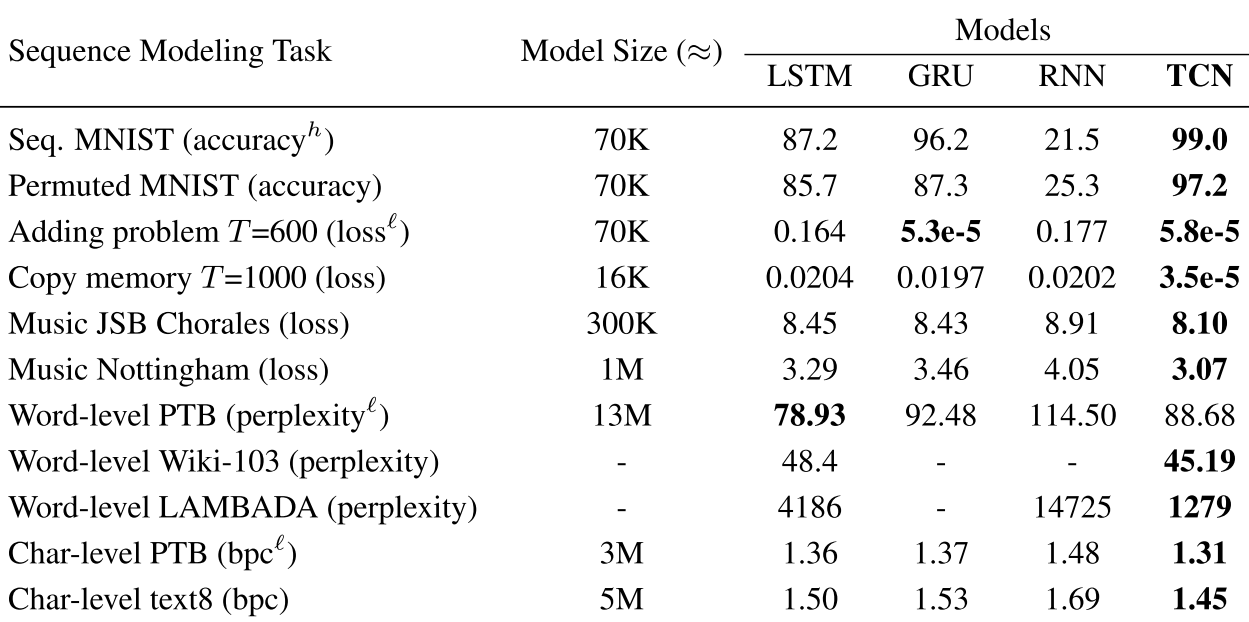
\includegraphics[width=1.0\textwidth]{../img/results}
\caption{Comparison of TCN and standard RNN. The TCNs had tuned $k$, $d$, number of layers, gradient clipping. They did a grid search over optimizer, recurrent drop, learning rate, gradient clipping, and initial forget-gate bias. Both TCN and RNN should have similar number of parameters in the comparisons.}
\label{fig:results}
\end{figure}

\begin{figure}[h!]
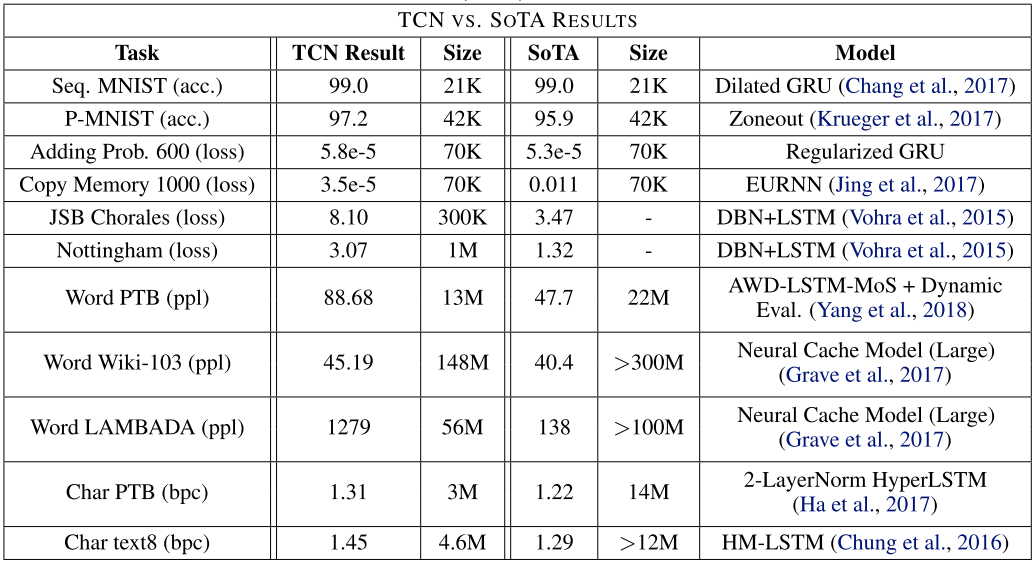
\includegraphics[width=1.0\textwidth]{../img/sota}
\caption{Comparison of TCN and State-of-the-art results on the datasets.}
\label{fig:sota}
\end{figure}

\section{Conclusion}
The results strongly suggest that the generic TCN architecture with minimal tuning outperforms canonical recurrent architectures across a broad variety of sequence modeling tasks that are commonly used to benchmark the performance of recurrent architectures themselves. 

TCN excel at the adding and copy tasks where they achieve perfect accuracy. The ability to memorize information from distant past has been evaluated on the copy task with increasing length of the sequence between the input that needs to be remembered and the output where it needs to be reproduced. TCNs consistently converged to 100\% accuracy for all sequence lengths, whereas LSTMs and GRUs of the same size quickly degenerated to random guessing as the sequence length T grows.



\clearpage

\begin{thebibliography}{0}
  \bibitem[1]{cit:nn} Nielsen, Michael A. Neural networks and deep learning. Vol. 25. USA: Determination press, 2015.
  
  \bibitem[2]{cit:cnn} "CS231n Convolutional Neural Networks for Visual Recognition" \url{http://cs231n.github.io/convolutional-networks/}
  
  \bibitem[3]{cit:lstm} Olah, Christopher. "Understanding lstm networks." (2015). \url{http://colah.github.io/posts/2015-08-Understanding-LSTMs/}
  
  \bibitem[4]{cit:tcn} Bai, Shaojie, J. Zico Kolter, and Vladlen Koltun. "An empirical evaluation of generic convolutional and recurrent networks for sequence modeling." arXiv preprint arXiv:1803.01271 (2018). \url{https://arxiv.org/abs/1803.01271} 
  
  Code: \url{https://github.com/locuslab/TCN}
  
  


  
  
  
  
  \end{thebibliography}


 
\end{document}
